\chapter{核心候选蛋白的机制解析与功能验证}

在前述章节中，本研究构建了Human-level与Immune-level双层蛋白必需性预测模型，并基于PES指标建立了跨层级比较框架。通过对Immune-level高分蛋白的系统筛选，本研究获得了一批在免疫情境中可能具有情境依赖特征的候选蛋白。然而，模型预测本身并不等同于生物学事实，其合理性必须通过机制层面的解释与功能对照加以验证。因此，本章围绕预测结果展开机制解析，旨在回答两个核心问题：其一，模型是否识别到了与氧化爆发-颗粒/溶酶体高负荷活化状态相对应的分子模块；其二，模型所提示的情境依赖特征是否能够在既有分子机制层面获得解释与支撑。

\section{免疫情境候选必需蛋白的功能关联分析与筛选结果}

中性粒细胞作为先天免疫系统的终末效应细胞，在功能执行过程中处于高度动态的应激环境之中。其吞噬体在形成后迅速酸化，pH可降至4.5--5.0；同时伴随NADPH氧化酶介导的ROS爆发以及大量颗粒融合与膜重塑过程。相关综述指出，中性粒细胞在分化与激活阶段均呈现出显著增强的溶酶体与颗粒系统活性，其蛋白水解与膜周转负荷远高于大多数体细胞 \cite{arocacrevilln2024neutrophils}。基于此，本文将后续实验所对应的生物学状态具体界定为急性炎症应答中以氧化爆发增强和颗粒/溶酶体功能负荷升高为特征的活化中性粒细胞状态，即氧化爆发-颗粒/溶酶体高负荷活化状态。因此，在这一状态下维持膜完整性、酸化动力学与蛋白降解效率的分子模块，很可能构成关键功能节点。

为验证模型所识别候选蛋白的生物学合理性，本研究对Immune-level高分蛋白进行了功能注释。结果显示，其功能并非随机分布，而是呈现出明显的聚集趋势。免疫情境候选必需蛋白中PES前10的蛋白列于表 \ref{tab:top_proteins}，其Immune-level得分普遍显著高于Human-level，提示这组蛋白在免疫情境中具有更强依赖性。结合前文定义，模型赋予的高分进一步印证，它们与氧化爆发-颗粒/溶酶体高负荷活化状态的核心功能需求密切相关，尤其集中于酸化、颗粒运输与溶酶体稳态维持等过程。

\begin{table}[htbp]
\centering
\caption{免疫情境中PES前10的候选必需蛋白}
\label{tab:top_proteins}
\begin{tabular}{lccc}
\toprule
\textbf{蛋白名称} & \textbf{Human-level PES} & \textbf{Immune-level PES} & \textbf{功能} \\
\midrule
ATP6V1B2 & 0.007 & 0.952 & 其他功能 \\
ATP6V1A & 0.450 & 0.940 & 其他功能 \\
PLBD1 (LyLAP) & 0.328 & 0.923 & 其他功能 \\
H2BC4 & 0.013 & 0.891 & 组蛋白 - 核心组蛋白H2B \\
H2BC7 & 0.013 & 0.891 & 组蛋白 - 染色质结构 \\
H2BC11 & 0.015 & 0.890 & 组蛋白 - 核心组蛋白H2B \\
H2BC21 & 0.012 & 0.888 & 组蛋白 - 染色质结构 \\
H2BC13 & 0.012 & 0.885 & 组蛋白 - 染色质结构 \\
\bottomrule
\end{tabular}
\end{table}

ATP6V1B2和ATP6V1A的Immune-level得分分别为0.952和0.940，均显著高于Human-level，提示它们在高应激免疫效应执行情境下具有较强的功能依赖性。ATP6V1A和ATP6V1B2是液泡型ATP酶（vacuolar-type ATPase, V-ATPase）复合体V1结构域的核心亚基，负责ATP水解和质子转运。V-ATPase通过ATP水解提供能量，将质子泵入溶酶体等细胞内腔室，维持低pH环境，这是溶酶体酸化的关键步骤\cite{chen2025emerging}。

在免疫细胞中，V-ATPase介导的酸化过程对溶酶体酶的激活和病原清除至关重要。对于中性粒细胞，V-ATPase的活性不仅确保酸化过程，还支持吞噬体成熟和与ROS的协同作用。因此，V-ATPase的功能异常会导致免疫反应效率下降，影响病原的清除\cite{kim2025failure}。

特别是ATP6V1B2，其在Immune-level中的得分为0.952，而在Human-level中仅为0.007，呈现出显著的跨层级差异。这一差异提示ATP6V1B2在不同生理环境下可能承担不同的功能角色。具体而言，Human-level中较低的PES值可能反映其在基础生理条件下的低依赖性，而Immune-level中的高得分则反映其在上述高应激情境中的依赖程度明显升高。这种跨层级的PES差异，可能与活化中性粒细胞在氧化爆发增强和颗粒/溶酶体负荷升高背景下对酸化动力学的特殊需求相关。在这一情境中，ATP6V1B2可能通过促进更高效的质子泵装配和质子转运，增强酸性环境的形成，从而促进溶酶体酶的激活和底物降解。

PLBD1（也称为LyLAP）在免疫激活背景下的高得分（Immune-level PES=0.923）也支持其与中性粒细胞颗粒/溶酶体稳态维持密切相关。与溶酶体膜稳态相关的功能在上述高应激情境中表现出较强依赖特征，其作用机制也在近年来的研究中得到了较为详细的证实\cite{jain2025leucine}。

此外，若干组蛋白家族成员（如H2BC4、H2BC7、H2BC11、H2BC21和H2BC13）在Immune-level中获得高分，也提示它们可能参与中性粒细胞特有的NETs形成过程。NETs是中性粒细胞在遇到病原体或炎症刺激时，通过一种不同于经典吞噬和脱颗粒的途径，将去凝集的染色质及其相关蛋白质网状释放到胞外形成的防御结构。这种网状结构由DNA、组蛋白及多种抗菌蛋白（如髓过氧化物酶和弹性蛋白酶）组成，能够物理捕获并杀灭微生物，从而扩展中性粒细胞的杀菌能力\cite{shahzad2025neutrophil}。组蛋白不仅是NETs结构的核心，还可通过后续修饰（如瓜氨酸化）调控NETs的形成 \cite{hamam2019histone}。在免疫激活条件下，组蛋白的修饰和去凝集作用尤为重要，也从侧面体现出它们在中性粒细胞免疫反应中的高必需性。

这些机制性研究与本研究观察到的Immune-level高评分高度一致：在静息状态下，这些组蛋白的Human-level PES得分较低，但在应激激活条件下显著升高，反映出它们在NETs形成这一中性粒细胞特有免疫功能中的依赖性增强。换言之，Immune-level模型不仅捕捉了这些蛋白的存在，还揭示了它们在特定激活背景下功能权重的动态提升，这与NETosis过程中染色质和组蛋白重要性的机制理解相互呼应。

综合来看，这些结果进一步支持了Immune-level模型在识别免疫情境候选依赖蛋白方面的准确性与可靠性。

\section{LyLAP（PLBD1）的机制解析与模型验证意义}

PLBD1（Phospholipase B Domain-containing 1）长期以来基于序列同源性注释为类磷脂酶B蛋白，但近年来的系统生化实验与结构解析重新界定了其生物学功能。研究证明，该蛋白并非作用于磷脂底物，而是一种LyLAP\cite{jain2025leucine}。LyLAP属于N-末端亲核试剂（Ntn）水解酶家族，其催化活性严格依赖于核心残基Cys228。图 \ref{fig:plbd1_structure} 概括了LyLAP的功能重定义、酸性激活过程以及对溶酶体内疏水跨膜片段的过程性修剪机制。

\begin{figure}[!htbp]
    \centering
    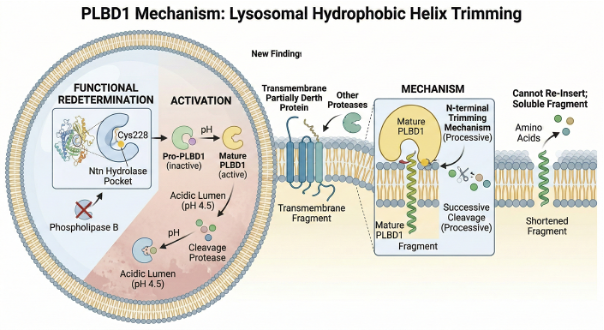
\includegraphics[width=0.98\linewidth]{figures/PLBD1.png}
    \caption[LyLAP的机制示意图]{LyLAP的机制示意图。图中展示了PLBD1从“类磷脂酶B”到LyLAP的功能重定义、其在酸性溶酶体环境中的成熟激活过程，以及成熟LyLAP对跨膜蛋白降解后残留疏水片段进行N端过程性修剪并防止其重新插入膜结构的机制。}
    \label{fig:plbd1_structure}
\end{figure}

由图 \ref{fig:plbd1_structure} 左侧可见，PLBD1的关键认识更新在于其催化口袋虽具有Ntn水解酶家族特征，但并不支持其作为经典磷脂酶B发挥作用。相反，在溶酶体酸性条件下（pH 4.5），PLBD1经历自催化切割并去除位于N端的抑制性肽段（L209-H227），在组织蛋白酶协同作用下转变为成熟LyLAP，从而暴露出能够高效结合底物的催化口袋。这种pH依赖激活特性提示其功能与溶酶体环境高度耦合，而并非普遍存在于细胞质或中性条件下的蛋白水解系统。

生理底物并非一般可溶性蛋白，而是来源于跨膜蛋白降解过程中残留的疏水 $\alpha$-螺旋片段。在溶酶体内，跨膜蛋白经多种蛋白酶初步切割后，往往残留较长的疏水跨膜区段。这些肽段由于疏水性强，具有重新插入脂质双层的能力，从而扰乱膜结构稳定性。

图 \ref{fig:plbd1_structure} 右侧进一步显示，成熟LyLAP并不是一次性将底物完全裂解，而是通过N端过程性修剪机制持续切除底物的N端氨基酸，逐步缩短疏水链长度，直至其失去重新嵌入膜结构的能力，最终转化为可溶性短肽和氨基酸。为展示这种底物选择性的结构基础，图~\ref{fig:LLL_AMC} 与图~\ref{fig:Gly_AMC} 分别给出了LyLAP与LLL-AMC、Gly-AMC的分子对接结果。

\begin{figure}[!htbp]
    \centering
    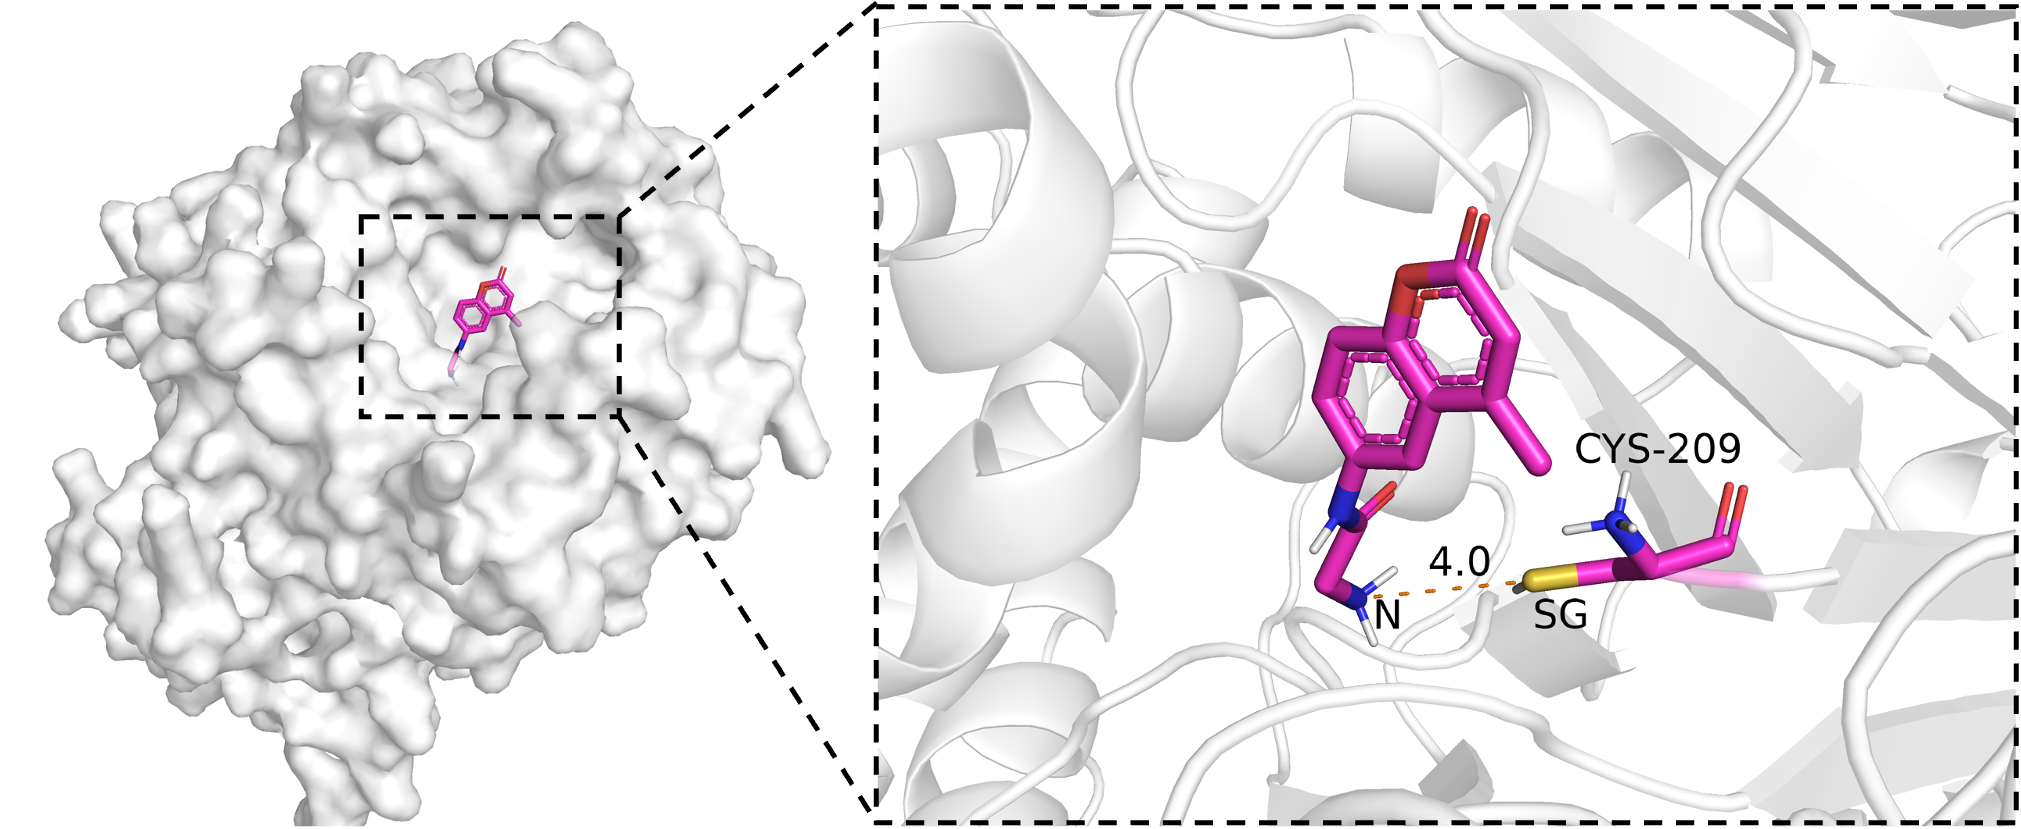
\includegraphics[width=0.88\linewidth]{figures/LLL-AMC.png}
    \caption[LyLAP与LLL-AMC底物的分子对接结果]{LyLAP与LLL-AMC底物的分子对接结果。图中显示疏水性底物LLL-AMC在LyLAP催化口袋中的结合构象，提示亮氨酸富集的N端基序能够与口袋形成稳定相互作用。}
    \label{fig:LLL_AMC}
\end{figure}
\begin{figure}[!htbp]
    \centering
    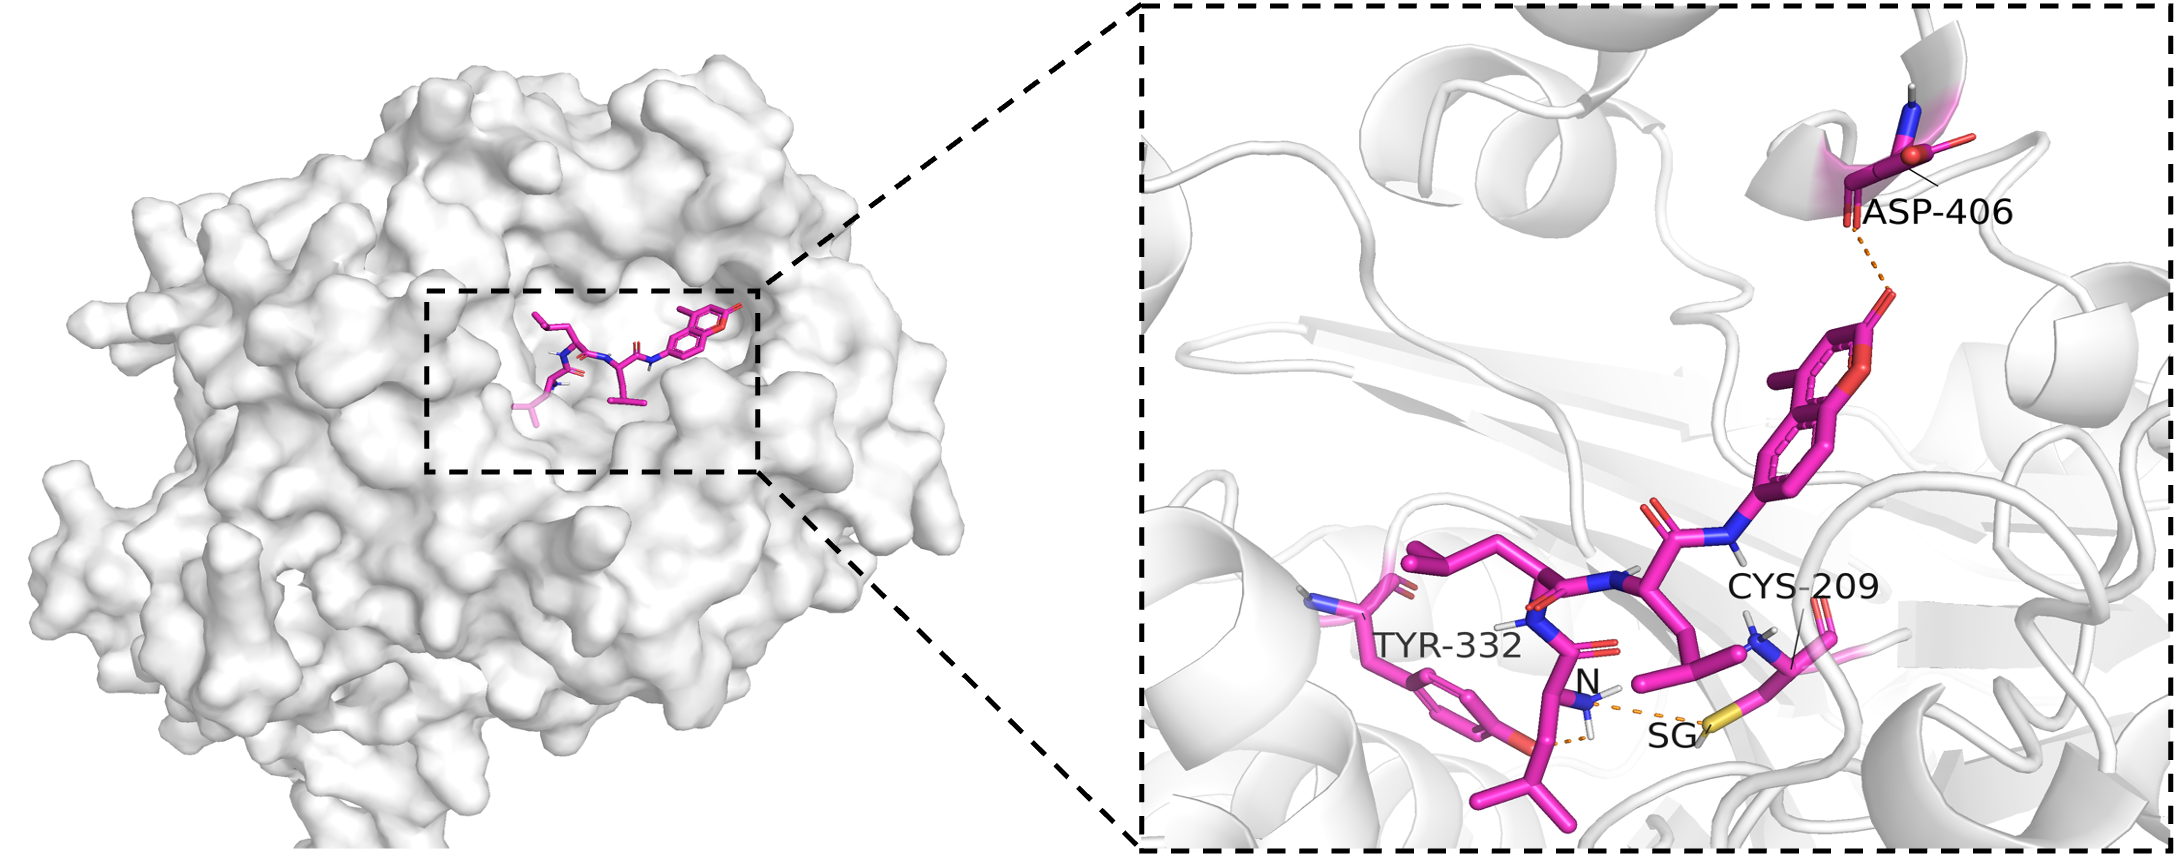
\includegraphics[width=0.88\linewidth]{figures/Gly-AMC.png}
    \caption[LyLAP与Gly-AMC底物的分子对接结果]{LyLAP与Gly-AMC底物的分子对接结果。图中展示了Gly-AMC在催化口袋中的结合姿态，其较弱的疏水嵌合特征与较低亲和倾向相一致。}
    \label{fig:Gly_AMC}
\end{figure}
\FloatBarrier

由图~\ref{fig:LLL_AMC} 可见，LLL-AMC的N端富含亮氨酸（Leu），具备强疏水性，与LyLAP催化口袋（CYS-209）形成了较强亲和作用，因此二者结合更为稳固。相比之下，图~\ref{fig:Gly_AMC} 所示的Gly-AMC由于其N端氨基酸为甘氨酸（Gly），较小且极性的特征使其不如亮氨酸那样稳定插入LyLAP的疏水性催化口袋，因此呈现出较低亲和力。两种底物的对比反映出LyLAP对疏水性氨基酸具有更高亲和倾向。当LyLAP功能缺失时，研究观察到疏水肽段在溶酶体腔内显著积累，并伴随ESCRT-III复合体异常招募、溶酶体膜通透性增加以及去酸化现象，最终导致细胞生长受抑与溶酶体功能失衡。

中性粒细胞含有丰富的颗粒系统，并频繁发生颗粒—溶酶体融合及内吞事件，其跨膜蛋白降解负荷显著高于一般细胞类型。同时，ROS爆发可能进一步加剧膜结构的不稳定性。在此背景下，疏水跨膜肽段的积累风险明显增加，因此LyLAP在中性粒细胞中可能承担更为关键的稳态维持功能。

PLBD1在Human-level模型中的评分相对平缓，而在Immune-level模型中显著升高。这种跨层级评分差异与PIC框架所强调的情境依赖特征高度一致。因此，LyLAP的机制解析不仅验证了预测结果的合理性，也为双层模型识别策略提供了机制层面的支撑。

\section{ATP6V1B2的功能推断与实验验证}

ATP6V1B2属于V-ATPase V1结构域亚基。已有研究指出，在应激条件下，ABL1激酶可磷酸化ATP6V1B2的Y68位点，促进V1结构域与V0结构域的装配，从而增强质子转运效率并加速溶酶体酸化 \cite{song2025nonreceptor}。这一调控更接近装配动力学层面的调节，而非简单的表达水平变化。

\begin{figure}[!htbp]
    \centering
    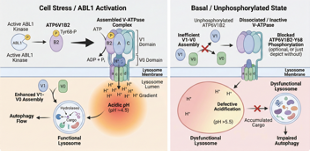
\includegraphics[width=0.98\linewidth]{figures/ATP6V1B2.png}
    \caption[ATP6V1B2介导V-ATPase装配与酸化调控的机制示意图]{ATP6V1B2介导V-ATPase装配与酸化调控的机制示意图。图中展示了细胞应激或ABL1激活条件下，ATP6V1B2被磷酸化后促进V1与V0结构域装配、增强溶酶体质子转运并维持酸性环境的过程；同时对比了基础状态下未磷酸化时V-ATPase装配不足、酸化受限及底物累积的情形。}
    \label{fig:atp6v1b2_mechanism}
\end{figure}

图 \ref{fig:atp6v1b2_mechanism} 进一步表明，ATP6V1B2的关键作用不在于决定V-ATPase是否存在，而在于决定其在应激条件下能否高效装配并形成足够的质子泵活性。于基础或未磷酸化状态下，V1与V0结构域装配不足，溶酶体pH维持能力较弱，底物清除效率下降；而在ABL1激活背景下，ATP6V1B2被磷酸化后可促进复合体装配，提高质子内流、增强酸化并维持自噬/溶酶体通量。对于中性粒细胞而言，吞噬后酸化的速度直接决定水解酶活化效率与杀菌能力。酸化延迟可能导致蛋白水解效率下降，并削弱ROS与水解酶系统的协同作用。因此，ATP6V1B2在氧化爆发-颗粒/溶酶体高负荷活化状态下可能成为酸化效率的关键调控节点。

为进一步评估ATP6V1B2是否呈现与上述高应激情境相关的依赖特征，本研究设计基于短发夹RNA（short hairpin RNA, shRNA）的功能干扰实验。考虑到原代中性粒细胞体外存活时间短且遗传操作困难，本文选用HL-60细胞作为中性粒细胞的体外替代体系，并以293T细胞作为非免疫来源对照体系。已有研究表明，PMA刺激可在HL-60体系中诱导NADPH氧化酶相关ROS生成，并在中性粒细胞样HL-60体系中更明确地触发氧化应激应答 \cite{muranaka2005mechanism,kuwabara2015nadph}。因此，本文在HL-60替代体系中施加PMA刺激，用以模拟氧化爆发-颗粒/溶酶体高负荷活化状态，从而近似再现氧化爆发增强及溶酶体/酸化负荷升高等关键功能特征；同时在293T细胞中设置平行处理，用于区分ATP6V1B2敲低所导致的普遍生长抑制与免疫情境相关的条件性依赖效应。

首先采用Western blot检测shRNA干扰后的蛋白水平变化。结果如图 \ref{fig:atp6v1b2_wb}(a) 与图 \ref{fig:atp6v1b2_wb}(b) 所示，在293T与HL-60两种细胞中，ATP6V1B2条带强度在敲低组均较对照组明显减弱，说明构建的干扰体系能够在两种细胞背景下稳定下调目标蛋白表达，为后续功能表型比较提供了基础。

\begin{figure}[!htbp]
    \centering
    \includegraphics[width=0.92\linewidth]{figures/wb.pdf}
    \caption[ATP6V1B2敲低后的Western blot检测]{ATP6V1B2敲低后的Western blot检测。图中展示了293T细胞与HL-60细胞中ATP6V1B2敲低后的Western blot结果，两种细胞中敲低组条带均较对照组减弱，表明shRNA可有效下调ATP6V1B2表达。}
    \label{fig:atp6v1b2_wb}
\end{figure}

在此基础上，进一步利用CCK8检测ATP6V1B2敲低对细胞活性的影响。结果如图 \ref{fig:atp6v1b2_cck8}(a) 与图 \ref{fig:atp6v1b2_cck8}(b) 所示，ATP6V1B2敲低对不同细胞背景的影响存在明显差异。在293T细胞中，敲低组细胞活性较对照组仅呈温和下降，无论是否给予PMA刺激，整体变化幅度均相对有限；相较之下，HL-60细胞在ATP6V1B2敲低后表现出更为明显的活性下降，且这一效应在PMA刺激条件下进一步增强。

具体而言，在HL-60细胞中，ATP6V1B2敲低后基础条件下细胞活性由对照组约95\%下降至约75\%，而在PMA刺激条件下进一步下降至约45\%，显著低于对应的阴性对照加PMA组；与此同时，阴性对照加PMA组与单独PMA组之间差异不显著，说明PMA处理本身并不是导致细胞活性下降的主要因素。相比之下，293T细胞中ATP6V1B2敲低后的活性虽有下降，但未见类似HL-60细胞中在PMA背景下进一步加重的抑制趋势。这表明ATP6V1B2敲低并不会在不同细胞类型中产生同等强度的广泛毒性，而更可能在接近中性粒细胞活化状态的HL-60体系中表现出更高的功能依赖性。

\begin{figure}[!htbp]
    \centering
    \includegraphics[width=0.98\linewidth]{figures/cck8.pdf}
    \caption[ATP6V1B2敲低后的CCK8细胞活性检测]{ATP6V1B2敲低后的CCK8细胞活性检测。图中展示了293T细胞与HL-60细胞在ATP6V1B2敲低及PMA处理后的细胞活性变化，其中HL-60细胞在ATP6V1B2敲低并联合PMA刺激时出现最显著的活性下降，而293T细胞中对应变化较弱，提示ATP6V1B2依赖性具有明显的细胞背景与应激状态相关性。}
    \label{fig:atp6v1b2_cck8}
\end{figure}
\FloatBarrier

上述结果与模型预测所揭示的跨层级PES差异高度一致。ATP6V1B2在Human-level中的评分极低，而在Immune-level中显著升高，提示其并非普遍意义上的基础生存必需蛋白，而是在特定免疫情境下承担更关键的功能。HL-60实验中观察到的“敲低效应在PMA刺激后显著增强”，恰好对应了氧化爆发-颗粒/溶酶体高负荷活化状态下对酸化动力学的额外需求；而293T细胞缺乏这一免疫效应背景，因此即使敲低ATP6V1B2，也仅表现为相对有限的活性下降。

综合而言，Western blot结果确认了ATP6V1B2干扰体系的有效性，CCK8结果则进一步支持ATP6V1B2在中性粒细胞样高应激活化背景下具有更强的条件性依赖特征。该结果不仅为ATP6V1B2作为免疫情境候选必需蛋白提供了初步实验支撑，也从功能层面验证了双层模型在区分基础生存依赖与情境特异依赖方面的判别能力。
